\noindent
\begin{minipage}[t]{0.26\textwidth}
    \vspace*{2.2cm}
    \noindent
    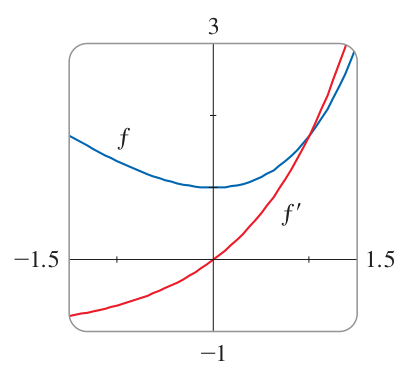
\includegraphics[width=\linewidth]{images/p0216_fig1.png}
    
    \vspace{4pt}
    \noindent
    \textbf{\textsf{\footnotesize HÌNH 8}}

    \vspace{2.4cm}
    \noindent
    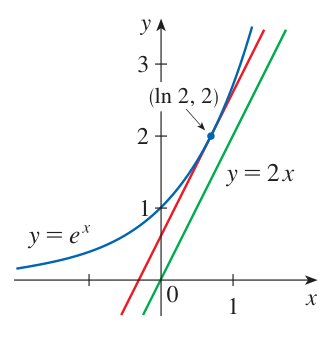
\includegraphics[width=0.95\linewidth]{images/p0216_fig2.png}
    
    \vspace{4pt}
    \noindent
    \textbf{\textsf{\footnotesize HÌNH 9}}
\end{minipage}%
\hfill
\begin{minipage}[t]{0.70\textwidth}
    Như vậy, hàm mũ $f(x) = e^x$ có tính chất là nó bằng chính đạo hàm của nó. Ý nghĩa hình học của thực tế này là hệ số góc của tiếp tuyến với đường cong $y = e^x$ tại điểm $(x, e^x)$ bằng chính tung độ $y$ của điểm đó (xem Hình 7).

    \vspace{0.6em}
    \noindent
    \textbf{\textsf{\color{stewartcyan}VÍ DỤ 8}}\quad Nếu $f(x) = e^x - x$, hãy tìm $f'$ và $f''$. So sánh đồ thị của $f$ và $f'$.

    \vspace{0.3em}
    \noindent
    \textbf{\textsf{\color{stewartcyan}LỜI GIẢI}}\quad Sử dụng Quy tắc hiệu, ta có
    \[
    f'(x) = \frac{d}{dx}(e^x - x) = \frac{d}{dx}(e^x) - \frac{d}{dx}(x) = e^x - 1
    \]
    Trong Mục 2.8, chúng ta đã định nghĩa đạo hàm cấp hai là đạo hàm của $f'$, do đó
    \[
    f''(x) = \frac{d}{dx}(e^x - 1) = \frac{d}{dx}(e^x) - \frac{d}{dx}(1) = e^x
    \]
    Hàm số $f$ và đạo hàm $f'$ của nó được vẽ trong Hình 8. Chú ý rằng $f$ có một tiếp tuyến nằm ngang khi $x = 0$; điều này tương ứng với việc $f'(0) = 0$. Cũng lưu ý rằng, khi $x > 0$, $f'(x)$ nhận giá trị dương nên $f$ đồng biến. Khi $x < 0$, $f'(x)$ nhận giá trị âm nên $f$ nghịch biến.\hfill{\color{stewartcyan}\rule{1.1ex}{1.1ex}}

    \vspace{0.8em}
    \noindent
    \textbf{\textsf{\color{stewartcyan}VÍ DỤ 9}}\quad Tại điểm nào trên đường cong $y = e^x$ thì tiếp tuyến song song với đường thẳng $y = 2x$?

    \vspace{0.3em}
    \noindent
    \textbf{\textsf{\color{stewartcyan}LỜI GIẢI}}\quad Vì $y = e^x$, ta có $y' = e^x$. Gọi hoành độ của điểm cần tìm là $a$. Khi đó hệ số góc của tiếp tuyến tại điểm đó là $e^a$. Tiếp tuyến này sẽ song song với đường thẳng $y = 2x$ nếu nó có cùng hệ số góc, tức là bằng 2. Cân bằng hai hệ số góc, ta được
    \[
    e^a = 2 \qquad\qquad a = \ln 2
    \]
    Do đó, điểm cần tìm là $(a, e^a) = (\ln 2, 2)$. (Xem Hình 9.)\hfill{\color{stewartcyan}\rule{1.1ex}{1.1ex}}
\end{minipage}

\vspace{1.5em}
\noindent
\begin{tikzpicture}[remember picture, x=1cm, y=1cm]
    \node[fill=stewartcyan, text=white, inner sep=3.5pt, anchor=west] (secnum) at (1.2, 0) {\fontsize{12}{14}\selectfont\textbf{\textsf{3.1}}};
    \node[anchor=west, inner sep=0pt] (sectitle) at ([xshift=0.6em]secnum.east) {\fontsize{14}{16}\selectfont\textbf{\textsf{\color{stewartcyan}Bài tập}}};
    
    \draw[stewartcyan, line width=0.8pt] (0, 0.18) -- (1.0, 0.18);
    \draw[stewartcyan, line width=0.8pt] (0, -0.18) -- (1.0, -0.18);
    
    \draw[stewartcyan, line width=0.8pt] ([xshift=0.7em, yshift=0.18cm]sectitle.east) -- (\linewidth, 0.18);
    \draw[stewartcyan, line width=0.8pt] ([xshift=0.7em, yshift=-0.18cm]sectitle.east) -- (\linewidth, -0.18);
\end{tikzpicture}

\vspace{0.8em}
\noindent
\begin{minipage}[t]{0.47\textwidth}
    \begin{enumerate}[label=\textbf{\arabic*.}, leftmargin=1.2em, itemsep=0.9em]
        \item 
        \begin{enumerate}[label=\textbf{(\alph*)}, leftmargin=1.5em, itemsep=0.3em]
            \item Số $e$ được định nghĩa như thế nào?
            \item Sử dụng máy tính cầm tay để ước lượng các giá trị của giới hạn
            \begin{center}
            $\displaystyle \lim_{h \to 0} \frac{2.7^h - 1}{h} \qquad \text{và} \qquad \lim_{h \to 0} \frac{2.8^h - 1}{h}$
            \end{center}
            chính xác đến hai chữ số thập phân. Bạn có thể rút ra kết luận gì về giá trị của $e$?
        \end{enumerate}

        \item 
        \begin{enumerate}[label=\textbf{(\alph*)}, leftmargin=1.5em, itemsep=0.3em]
            \item Hãy phác họa bằng tay đồ thị của hàm số $f(x) = e^x$, đặc biệt chú ý đến cách đồ thị cắt trục $y$. Hệ số góc của tiếp tuyến tại điểm đó bằng bao nhiêu?
            \item $f(x) = e^x$ và $g(x) = x^e$ thuộc những loại hàm số nào? So sánh các công thức tính đạo hàm của $f$ và $g$.
            \item Hàm số nào trong hai hàm số ở phần (b) tăng nhanh hơn khi $x$ rất lớn?
        \end{enumerate}
    \end{enumerate}
\end{minipage}%
\hfill
\begin{minipage}[t]{0.49\textwidth}
    \noindent
    \textbf{\textsf{\color{stewartcyan}3–34}}\quad \textsf{Tính đạo hàm của các hàm số sau.}
    
    \vspace{0.6em}
    \noindent
    \begin{tabularx}{\linewidth}{@{}p{0.48\linewidth}@{\hspace{0.04\linewidth}}p{0.48\linewidth}@{}}
      \textbf{3.} $f(x) = 4x + 7$ & \textbf{4.} $g(t) = 5t + 4t^2$ \\[0.8em]
      \textbf{5.} $f(x) = x^{75} - x + 3$ & \textbf{6.} $g(x) = \frac{7}{4}x^2 - 3x + 12$ \\[0.9em]
      \textbf{7.} $f(t) = -22e^t$ & \textbf{8.} $F(t) = t^3 + e^3$ \\[0.8em]
      \textbf{9.} $W(v) = 1.8v^{-3}$ & \textbf{10.} $r(z) = z^{-5} - z^{1/2}$ \\[0.8em]
      \textbf{11.} $f(x) = x^{3/2} + x^{-3}$ & \textbf{12.} $V(t) = t^{-3/5} + t^4$ \\[0.8em]
      \textbf{13.} $s(t) = \dfrac{1}{t} + \dfrac{1}{t^2}$ & \textbf{14.} $r(t) = \dfrac{a}{t^2} + \dfrac{b}{t^4}$ \\[1.2em]
      \textbf{15.} $y = 2x + \sqrt{x}$ & \textbf{16.} $h(w) = \sqrt{2}\,w - \sqrt{2}$
    \end{tabularx}
\end{minipage}

\vfill
\noindent
\rule{\textwidth}{0.3pt}\\[2pt]
\centerline{\tiny\textsf{\color{stewartgray}Copyright 2021 Cengage Learning. Bản dịch tiếng Việt phục vụ mục đích học tập và nghiên cứu.}}
